\begin{pastexam}[label={px:gw3-100-ds-01}]{關務三等資訊處理 100 年 第一題}
（申論；30 分）

下圖為二元搜尋樹（binary search tree），請回答下列問題：（每小題 5 分，共 30 分）
\begin{center}
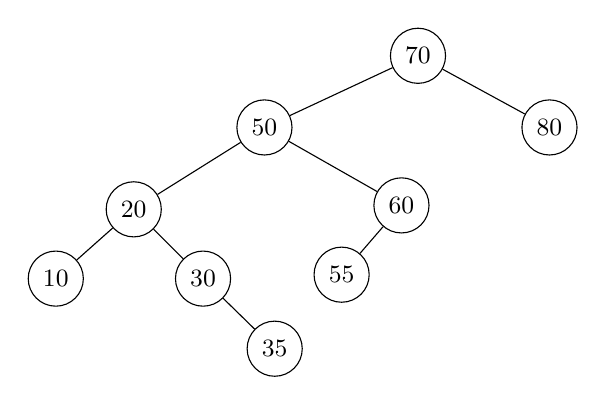
\begin{tikzpicture}[x=1cm,y=1cm,every node/.style={circle,draw,minimum size=7mm,inner sep=0pt,font=\small}]
\node (70) at (4.60,0.00) {70};
\node (50) at (2.65,-0.91) {50};
\node (80) at (6.27,-0.91) {80};
\node (20) at (0.99,-1.95) {20};
\node (60) at (4.39,-1.90) {60};
\node (10) at (0.00,-2.83) {10};
\node (30) at (1.87,-2.83) {30};
\node (55) at (3.63,-2.78) {55};
\node (35) at (2.78,-3.72) {35};
\draw (70)--(50); \draw (70)--(80); \draw (50)--(20); \draw (50)--(60);
\draw (20)--(10); \draw (20)--(30); \draw (60)--(55); \draw (30)--(35);
\end{tikzpicture}
\end{center}
\begin{itemize}[leftmargin=2.2em]
\item[㈠] 35 的 successor 為何？
\item[㈡] 50 的 successor 為何？
\item[㈢] 寫出 Entry<E> successor(Entry<E> e) 的 pseudo code。
\item[㈣] 寫出 preorder traversal。
\item[㈤] 寫出 postorder traversal。
\item[㈥] 寫出 inorder traversal。
\end{itemize}
\end{pastexam}

\begin{pastsoln}
答案：㈠ 50；㈡ 55；㈣ 70, 50, 20, 10, 30, 35, 60, 55, 80；㈤ 10, 35, 30, 20, 55, 60, 50, 80, 70；㈥ 10, 20, 30, 35, 50, 55, 60, 70, 80。

樹的結構：70 的左子是 50、右子是 80；50 的左子 20、右子 60；20 的左子 10、右子 30；30 的右子 35；60 的左子 55。 successor（後繼）是
中序順序中的下一個，也就是比它大的鍵中最小的（資結書第~9.1~節）。

\textbf{㈠ 35 的後繼}。 35 沒有右子樹，所以往上找：35 是 30 的右子、30 是 20 的右子，繼續往上；20 是 50 的\textbf{左}子，停下，後繼是 50。
（從 35 往上到第一個「自己在它左子樹裡」的祖先。）對照 ㈥：35 的下一個是 50。

\textbf{㈡ 50 的後繼}。 50 有右子樹（根是 60），後繼是右子樹的最小值：從 60 一路往左走到 55，55 沒有左子，後繼是 55。

\textbf{㈢}。 照 Java \texttt{TreeMap} 的寫法，每個 \texttt{Entry} 有 \texttt{left}、\texttt{right}、\texttt{parent} 三個指標（資結書虛擬碼~9.4）：
\begin{pseudo}[unbreakable]{\texttt{Entry<E> successor(Entry<E> e)}}
\Function{successor}{$e$}
    \If{$e = \NIL$}
        \State \Return $\NIL$
    \ElsIf{$e.\mathit{right} \ne \NIL$} \Comment{情況一：有右子樹}
        \State $p \gets e.\mathit{right}$
        \While{$p.\mathit{left} \ne \NIL$}
            \State $p \gets p.\mathit{left}$
        \EndWhile
        \State \Return $p$ \Comment{右子樹的最小值}
    \Else \Comment{情況二：沒有右子樹，往上找}
        \State $p \gets e.\mathit{parent}$；$c \gets e$
        \While{$p \ne \NIL$ \AND $c = p.\mathit{right}$}
            \State $c \gets p$；$p \gets p.\mathit{parent}$
        \EndWhile
        \State \Return $p$ \Comment{$\NIL$ 表示 $e$ 是最大值，沒有後繼}
    \EndIf
\EndFunction
\end{pseudo}
\textbf{正確性}：情況一，右子樹的鍵都比 $e$ 大，而 $e$ 和右子樹之間沒有其他鍵（祖先中比 $e$ 大的，也比整棵右子樹大），所以後繼是右子樹最小
（最左）的節點。 情況二，往上走時只要自己是父節點的右子，父節點就比自己小，要繼續；第一次從左邊上來的那個祖先 $p$，$e$ 在它的左子樹中，$p$
是比 $e$ 大的最小鍵。 時間 $O(h)$。 追蹤 ㈠：$e = 35$，$p = 30$，$35 = 30.\mathit{right}$；$c = 30$、$p = 20$，$30 = 20.\mathit{right}$；$c = 20$、
$p = 50$，$20$ 是 $50$ 的左子，停，傳回 $50$。

\textbf{㈣ 前序}（根、左、右）：70, 50, 20, 10, 30, 35, 60, 55, 80。

\textbf{㈤ 後序}（左、右、根）：10, 35, 30, 20, 55, 60, 50, 80, 70。

\textbf{㈥ 中序}（左、根、右）：10, 20, 30, 35, 50, 55, 60, 70, 80。 二元搜尋樹的中序一定是由小到大（資結書定理~9.1），可以拿來檢查。
\end{pastsoln}
